\documentclass[acmsmall,screen,review]{acmart}

%% Rights management information.  This information is sent to you
%% when you complete the rights form.  These commands have SAMPLE
%% values in them; it is your responsibility as an author to replace
%% the commands and values with those provided to you when you
%% complete the rights form.
\setcopyright{acmcopyright}
% \copyrightyear{2021}
\acmYear{2021}
\acmDOI{10.1145/1122445.1122456}


%%
%% These commands are for a JOURNAL article.
\acmJournal{TOMS}
\acmVolume{?}
\acmNumber{?}
\acmArticle{?}
\acmMonth{5}

\usepackage{bm}
% \usepackage{amssymb}
\usepackage{amsmath}   %use ams math descriptions
\usepackage{amsfonts}  %use ams fonts
\usepackage{amsthm}
\usepackage{booktabs}
\usepackage{graphicx} % more modern
\usepackage{epstopdf}
%\usepackage{subfigure}
\usepackage{threeparttable}
% \usepackage{algorithm2e}
\usepackage{algorithm}
\usepackage{algorithmic}
% \usepackage{algpseudocode}
\usepackage{caption}
\usepackage{subcaption}

%%
%% Submission ID.
%% Use this when submitting an article to a sponsored event. You'll
%% receive a unique submission ID from the organizers
%% of the event, and this ID should be used as the parameter to this command.
%%\acmSubmissionID{123-A56-BU3}

%%
%% The majority of ACM publications use numbered citations and
%% references.  The command \citestyle{authoryear} switches to the
%% "author year" style.
%%
%% If you are preparing content for an event
%% sponsored by ACM SIGGRAPH, you must use the "author year" style of
%% citations and references.
%% Uncommenting
%% the next command will enable that style.
% \citestyle{acmauthoryear}

%%
%% end of the preamble, start of the body of the document source.
\begin{document}

%%
%% The "title" command has an optional parameter,
%% allowing the author to define a "short title" to be used in page headers.
\title[Algorithm xxxx: KCC: A MATLAB Package for K-means-based Consensus Clustering]{Algorithm xxxx: KCC: A MATLAB Package for K-means-based Consensus Clustering}

%%
%% The "author" command and its associated commands are used to define
%% the authors and their affiliations.
%% Of note is the shared affiliation of the first two authors, and the
%% "authornote" and "authornotemark" commands
%% used to denote shared contribution to the research.
% \author{Hao Lin}
% \orcid{0000-0002-1921-3036}
% \email{linh@in.tum.de}
% \affiliation{%
%   \institution{Department of Informatics, Technical University of Munich}
%   \streetaddress{Boltzmannstr. 3}
%   \city{Garching}
%   \postcode{85748}
%   \country{Germany}
% }

% \author{Hongfu Liu}
% \email{hongfuliu@brandeis.edu}
% \affiliation{%
%   \institution{Michtom School of Computer Science, Brandeis University}
%   \streetaddress{415 South St}
%   \city{Waltham}
%   \state{MA}
%   \postcode{02453}
%   \country{USA}
% }

% \author{Junjie Wu}
% \authornote{Corresponding Author}
% \email{wujj@buaa.edu.cn}
% \affiliation{%
%   \institution{School of Economics and Management, Beihang University}
%   \streetaddress{37 Xueyuan Rd}
%   \city{Haidian District}
%   \state{Beijing}
%   \postcode{100191}
%   \country{China}
% }

% \author{Hong Li}
% \email{hong_lee@buaa.edu.cn}
% \affiliation{%
%   \institution{School of Economics and Management, Beihang University}
%   \streetaddress{37 Xueyuan Rd}
%   \city{Haidian District}
%   \state{Beijing}
%   \postcode{100191}
%   \country{China}
% }

% \author{Stephan Günnemann}
% \email{guennemann@in.tum.de}
% \affiliation{%
%   \institution{Department of Informatics, Technical University of Munich}
%   \streetaddress{Boltzmannstr. 3}
%   \city{Garching}
%   \postcode{85748}
%   \country{Germany}
% }

% \thanks{Dr. Hao Lin's work was partially supported by Sino-German (CSC-DAAD) Postdoc Scholarship Program under CSC (China Scholarship Council) Grant 201906020375 and DAAD (Deutscher Akademischer Austauschdienst) Grant 57531629.}

%%
%% By default, the full list of authors will be used in the page
%% headers. Often, this list is too long, and will overlap
%% other information printed in the page headers. This command allows
%% the author to define a more concise list
%% of authors' names for this purpose.
\renewcommand{\shortauthors}{Lin et al.}

%%
%% The abstract is a short summary of the work to be presented in the
%% article.
% \begin{abstract}
%   Consensus clustering is gaining increasing attention for its high quality and robustness. In particular, $K$-means-based Consensus Clustering (KCC) converts the usual computationally expensive problem to a classic $K$-means clustering with generalized utility functions, bringing potentials for large-scale data clustering on different types of data. Although previous publications demonstrated KCC's applicability and generalizability, implementing this method is challenging, and has seldom been discussed in prior work. To fill this gap, we present a MATLAB package, KCC, that implements the $K$-means-based Consensus Clustering framework, for easy use and extension in both academy and industry. The KCC package not only achieves the efficiency, effectiveness, and generalizability merits inherited from the KCC method, but also reduces the computation time and space complexity by further addressing issues in implementation. The sample usage of the KCC package is also included to show its usability on extensive real-world data sets.
% \end{abstract}

%%
%% The code below is generated by the tool at http://dl.acm.org/ccs.cfm.
%% Please copy and paste the code instead of the example below.
%%
% \begin{CCSXML}
% <ccs2012>
%    <concept>
%        <concept_id>10002951.10003227.10003351.10003444</concept_id>
%        <concept_desc>Information systems~Clustering</concept_desc>
%        <concept_significance>500</concept_significance>
%        </concept>
%    <concept>
%        <concept_id>10010147.10010257.10010321.10010333</concept_id>
%        <concept_desc>Computing methodologies~Ensemble methods</concept_desc>
%        <concept_significance>500</concept_significance>
%        </concept>
%    <concept>
%        <concept_id>10002950.10003705.10003708</concept_id>
%        <concept_desc>Mathematics of computing~Statistical software</concept_desc>
%        <concept_significance>500</concept_significance>
%        </concept>
%  </ccs2012>
% \end{CCSXML}

% \ccsdesc[500]{Information systems~Clustering}
% \ccsdesc[500]{Computing methodologies~Ensemble methods}
% \ccsdesc[500]{Mathematics of computing~Statistical software}

%%
%% Keywords. The author(s) should pick words that accurately describe
%% the work being presented. Separate the keywords with commas.
% \keywords{Consensus clustering, $K$-means, utility function, MATLAB}


%%
%% This command processes the author and affiliation and title
%% information and builds the first part of the formatted document.
\maketitle

\section[The KCC package]{The \textbf{KCC} package}\label{sec:package}
\begin{figure*}[!bt]
\centering
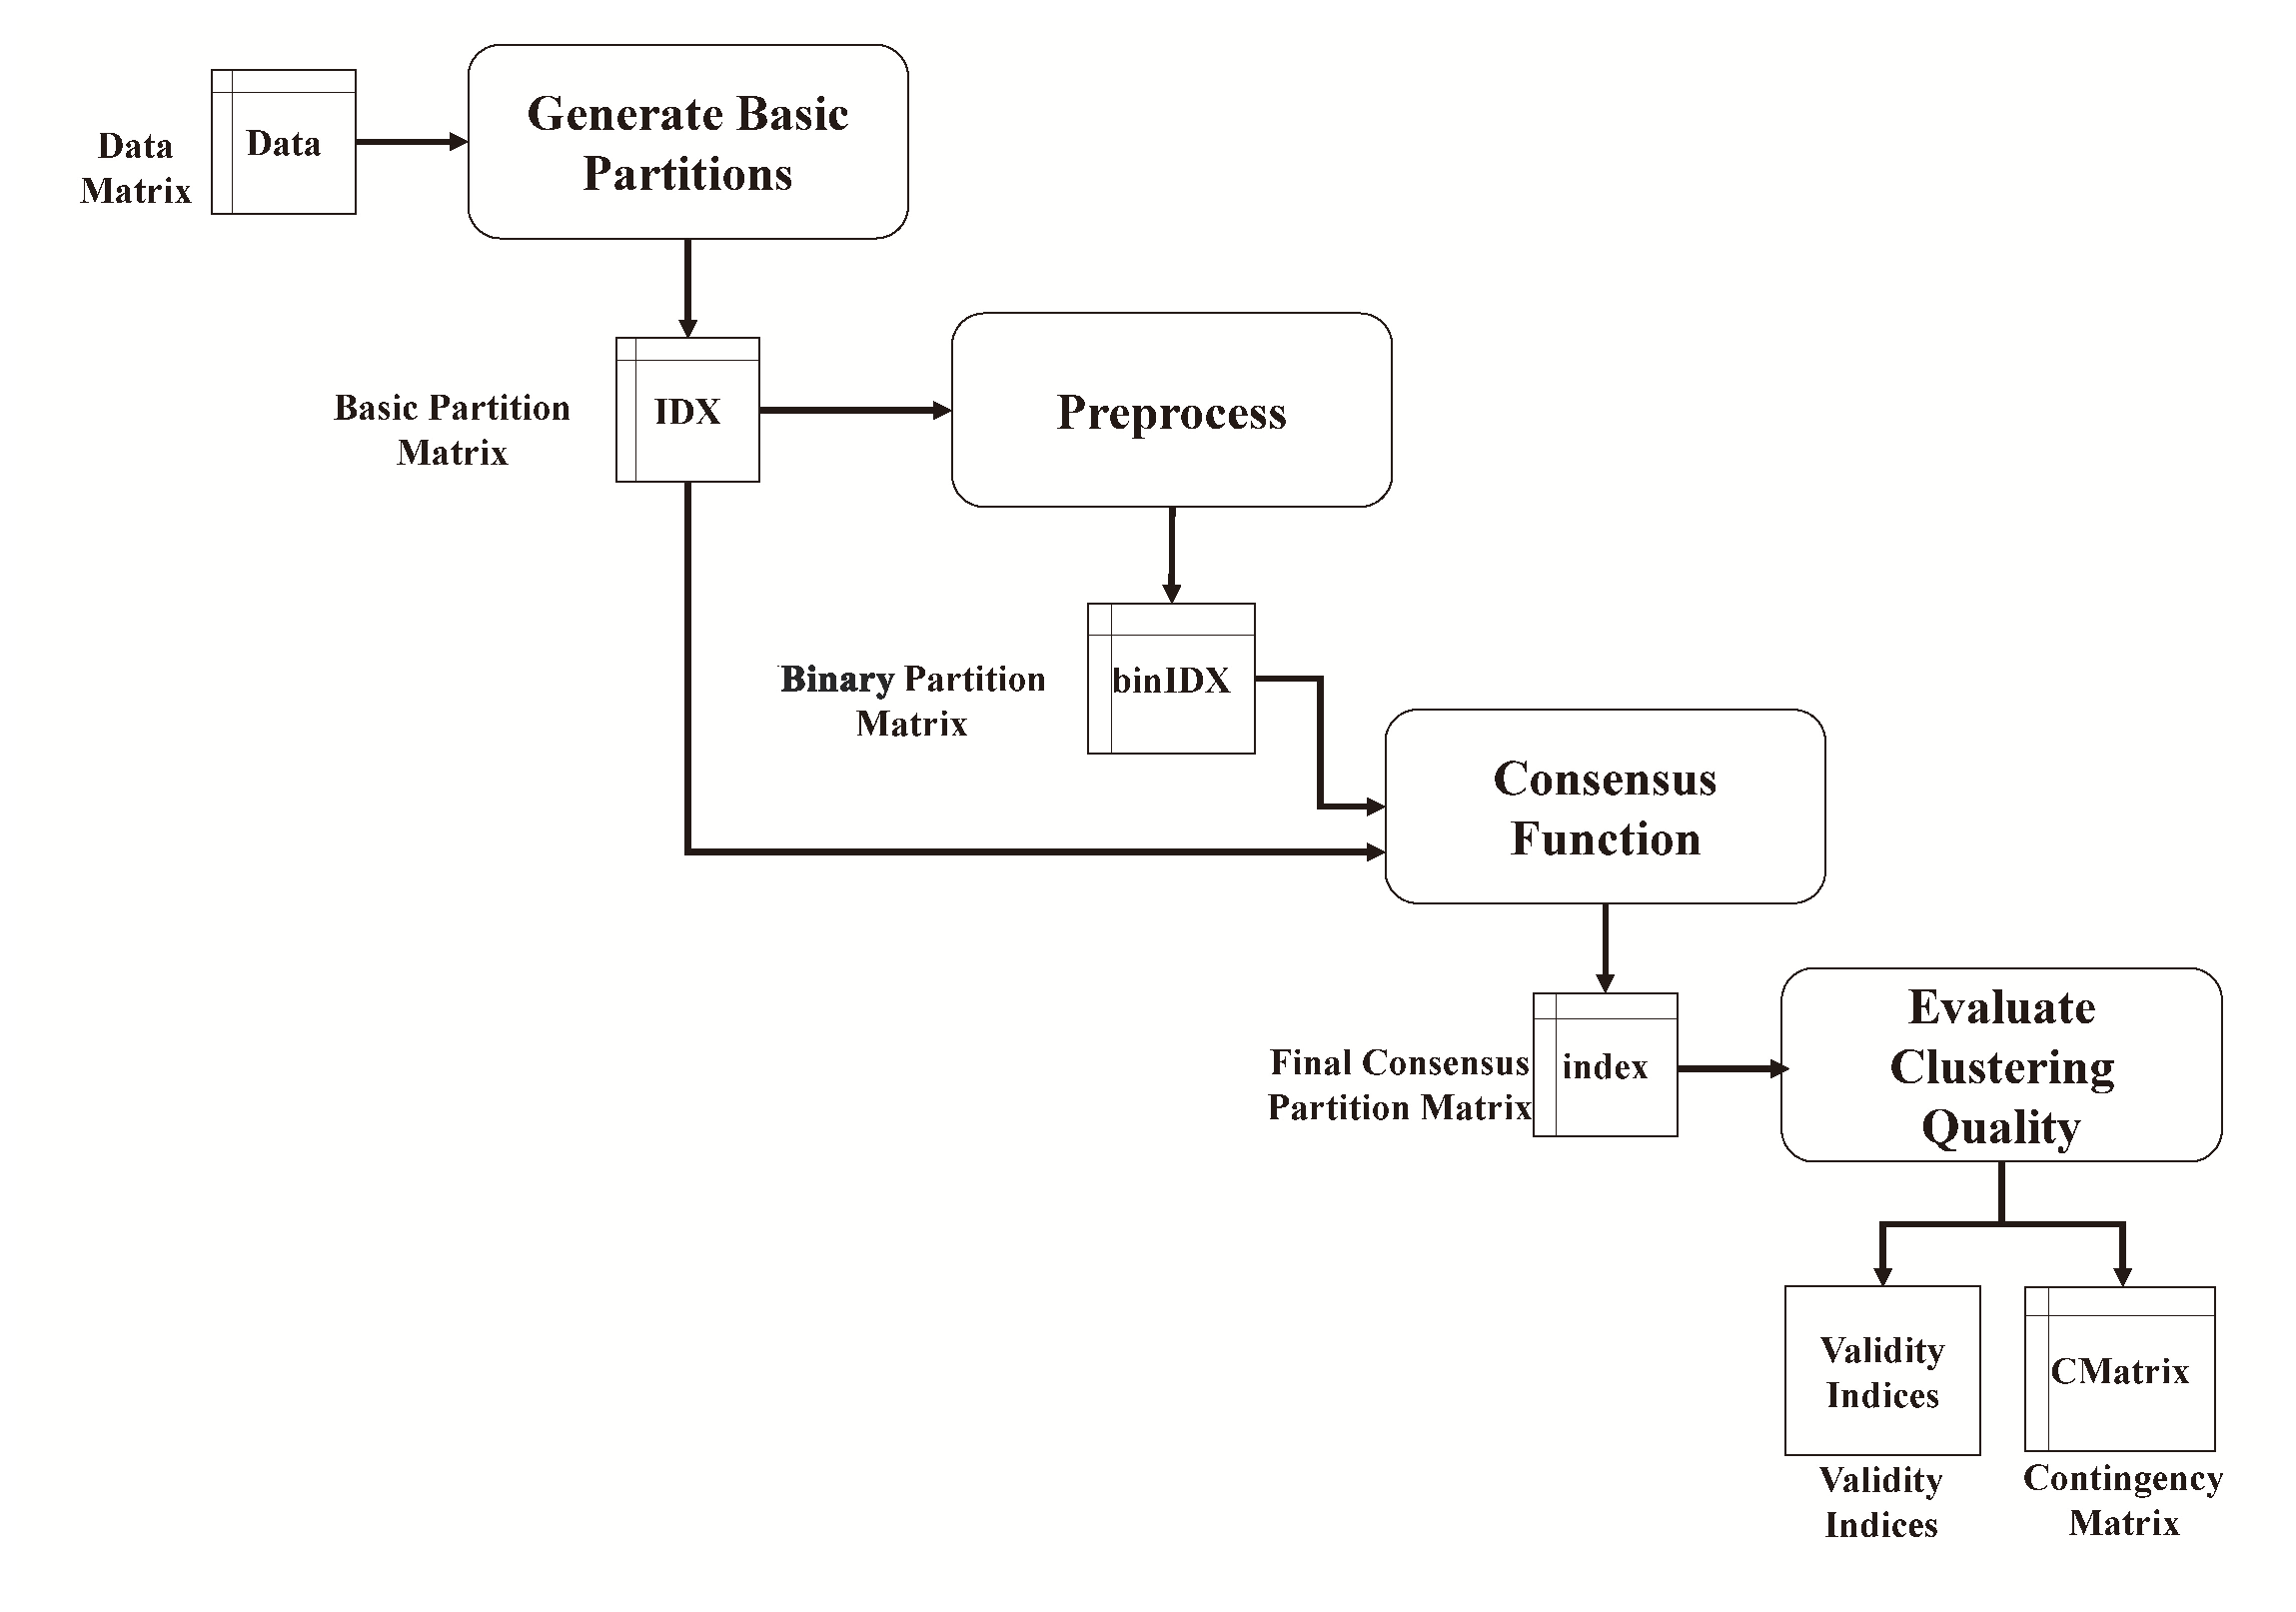
\includegraphics[width=0.85\textwidth]{fig/soft.eps}
\caption{Diagram of \textbf{KCC} package.}\label{fig:soft} % \label should be placed after \caption
\end{figure*}

This section presents a systematic MATLAB \textbf{KCC} package that implements the KCC method described in Section~\ref{sec:cc}, and tackles the issues in Section~\ref{sec:implementation}. Figure~\ref{fig:soft} illustrates the main functions of the \textbf{KCC} package, including basic partitions generation function, consensus clustering preprocessing function, consensus function, and clustering quality evaluation function. We can see from Figure~\ref{fig:soft} that, a real-world matrix \textsf{Data} is first input to generate a basic partition matrix \textsf{IDX}. The basic partition matrix is then input to a \textsf{Preprocess} function to produce the sparse representation of $\mathcal{X}^{(b)}$ as introduced in Section~\ref{sec:implementation}, i.e., the binary matrix \textsf{binIDX}. The binary matrix \textsf{binIDX}, along with the basic partition matrix \textsf{IDX} is the input of the final consensus clustering via a $K$-means heuristic, also known as consensus function, which produces a consensus partition matrix \textsf{index}. Lastly, the clustering quality is evaluated with an \textsf{exMeasure} function, which outputs several external validity indices and a contingency matrix.

\subsection{Basic partitions generation function} \label{subsec:gbp}
The first step of the KCC framework is to establish a collection of \textsf{r} basic partition results $\Pi=\{\pi_i\}, 1 \leq i \leq r$ . In the \textbf{KCC} package, the \textsf{BasicCluster\_RFS} and \textsf{BasicCluster\_RPS} functions are used to generate basic partition results. These two functions employ $K$-means as a base clustering algorithm, and uses the Random Feature Selection (RFS) strategy and the Random Parameter Selection (RPS) strategy as described in Section~\ref{subsec:bpgeneratestra}, respectively.

For the first basic partition generation function, namely \textsf{BasicCluster\_RFS} function, its input argument set consists of \textsf{Data}, \textsf{r}, \textsf{K}, \textsf{dist} and \textsf{nFeature}, which are the input data matrix, the predefined number of basic partitions, the predefined number of clusters in the basic partitions, the distance measure for $K$-means clustering in $p$-dimensional space, and the number of randomly selected partial features for RFS, respectively. In particular, \textsf{Data} is an \textsf{n} $\times$ \textsf{p} matrix of data, whose rows correspond to \textsf{n} observations, and columns correspond to \textsf{p} features. In RFS strategy, we set the number of clusters across all \textsf{r} basic partitions to a same value \textsf{K} for simplicity. The recommended value for the distance measure is \textsf{sqEuclidean} namely the squared Euclidean distance, and each centroid is the mean of the data points in a cluster. In the RFS process, a \textsf{nFeature} $\times$ \textsf{1} vector is sampled uniformly at random without replacement from the integers \textsf{1} to \textsf{p}, which forms the indices of the selected features.

For the \textsf{BasicCluster\_RPS} function, its input argument set consists of \textsf{Data}, \textsf{r}, \textsf{K}, \textsf{dist} and \textsf{RandKi}. Most of the function's input parameters are similar to those of \textsf{BasicCluster\_RFS}, except for that \textsf{RandKi} indicates different ways of setting the number of clusters in BPs. Recall that the RPS strategy is to randomly sample different number of cluster for each of the basic partitions. This random sampling strategy can only be activated by setting \textsf{RandKi} to 1 and under the condition of $\sqrt{n} > K$. More specifically, in the RPS strategy, a \textsf{r} $\times$ 1 vector is sampled uniformly at random with replacement from the values range from \textsf{K} to $\sqrt{n}$, each entry indicating the number of clusters for the corresponding basic partition. If \textsf{RandKi} is directly set to a \textsf{r} $\times$ \textsf{1} vector, this function produces \textsf{r} basic partitions of which the $i$-th BP's number of clusters is \textsf{RandKi(i)}. If \textsf{RandKi} is set to other values, this function produces \textsf{r} basic partitions with equal number (i.e., \textsf{K}) of clusters. 

The output produced from the above two functions is a \textsf{n} $\times$ \textsf{r} cluster labels matrix for \textsf{n} data points in \textsf{r} basic partitions, i.e., \textsf{IDX}. 
In practice, the \textsf{BasicCluster\_RFS} function is executed as follows:
\newline
\newline
\textsf{> IDX = BasicCluster\_RFS(Data, r, K, dist, nFeature)}
\newline
\newline
Similarly, the \textsf{BasicCluster\_RPS} function is executed as follows:
\newline
\newline
\textsf{> IDX = BasicCluster\_RPS(Data, r, K, dist, RandKi)}
\newline
\newline
It is worth noting that, both \textsf{BasicCluster\_RFS} and \textsf{BasicCluster\_RPS} are non-deterministic functions. Each call to each of them may yield a different output matrix IDX, due to the random feature sampling process in \textsf{RFS}, the random parameter selection process in \textsf{RPS}, and the random initializations in the $K$-means algorithm. In addition, users can implement their own basic partition generation strategies under the framework of \textbf{KCC} package, or directly import their existing basic partitions for later computation.

\subsection{Consensus clustering preprocessing function}\label{subsec:prepro}
With the basic partition matrix produced from Section~\ref{subsec:gbp}, some preprocessing techniques are required to produce the input for the final consensus clustering, as well as some auxiliary variables that can help to save memory and accelerate computations. The \textbf{KCC} package offers a \textsf{Preprocess} function for this purpose. The main input argument is basic partition matrix \textsf{IDX}, which can either be obtained using any user-defined base clustering algorithm or the \textsf{BasicCluster\_RFS/BasicCluster\_RPS} function. One of the main outputs of the \textsf{Preprocess} function is the data matrix \textsf{binIDX}, which is the sparse representation as introduced in Section~\ref{sec:implementation}, and serves as one important input to the final $K$-means algorithm. The \textsf{Preprocess} function can be called using the following command:
\newline
\newline
\textsf{> [Ki, sumKi, binIDX, missFlag, missMatrix, distance, Pvector, weight] = Preprocess(IDX, U, n, r, w, utilFlag)}
\newline
\newline
Input arguments of the \textsf{Preprocess} function contain \textsf{IDX}, \textsf{U}, \textsf{w} and \textsf{utilFlag}, which are the basic partition matrix, an argument related to the chosen utility function, a weight vector related to the objective function of the consensus clustering, and a flag indicator, respectively. The argument \textsf{U} is a \textsf{1} $\times$ \textsf{3} parameter cell array. More specifically, the first parameter \textsf{U\{1,1\}} defines the chosen type of the KCC utility function. It currently supports four different types of utility functions which correspond to four different $K$-means point-to-centroid distance functions, i.e., \textsf{`U\_c'} for Euclidean distance, \textsf{`U\_H'} for Kullback-Leibler Divergence, \textsf{`U\_cos'} for cosine similarity, and \textsf{`U\_Lp'} for Lp-norm. It is worth noting that \textsf{`U\_Lp'} corresponds the distance measure in $L_p$ spaces, which are function spaces defined using a natural generalization of the $p$-norm for finite-dimensional vector spaces. The second parameter \textsf{U\{1,2\}} is a parameter specifying the chosen form of the KCC utility function, i.e., \textsf{`std'} for the Standard Form, and \textsf{`norm'} for the Normalized Form. The third parameter \textsf{U\{1,3\}} is only required to be set when \textsf{`U\_Lp'} is chosen as the utility function. The settings of \textsf{p = 1}, \textsf{p = 2}, \textsf{p} $\rightarrow \infty$ correspond to the Manhattan distance, the euclidean distance and the chebyshev distance, respectively. The argument \textsf{w} is a \textsf{r} $\times$ \textsf{1} weight vector, of which each entry indicates the weight value assigned to each basic partition in the objective of consensus clustering. The last input argument \textsf{utilFlag} is a flag indicating whether to calculate utility function during the iterative computation of $K$-means.
% The \textsf{`std'} type uses a constant vector \textsf{w} as the weight vector of basic partitions while the \textsf{`norm'} type uses an adjusted weight vector.

The outputs of the \textsf{Preprocess} function contain \textsf{Ki}, \textsf{sumKi}, \textsf{binIDX}, \textsf{missFlag}, \textsf{missMatrix}, \textsf{distance}, \textsf{Pvector} and \textsf{weight}. The motivation of producing \textsf{Ki}, \textsf{sumKi}, and \textsf{binIDX} is to reduce memory usage, and accelerate the centroid and distance computation, which has been introduced in Section~\ref{sec:implementation}. The output variable \textsf{missFlag} $\in \{0, 1\}$ indicates whether the input \textsf{IDX} matrix contains incomplete basic partitions (IBPs) or not, and a mask matrix \textsf{missMatrix} represent the indices of the non-zero entries in \textsf{IDX} if there exists IBPs. The output variable \textsf{distance} determines the corresponding distance function to deal with the specific utility function defined by \textsf{U\{1,1\}}. The output vector \textsf{Pvector} is a \textsf{1} $\times$ \textsf{r} row vector calculated from the contingency matrix, i.e., $P^{(i)}_k$ in Equation~(\ref{equ:pvector}), which can later be used in calculating distance  and utility functions. The output vector \textsf{weight} is a \textsf{r} $\times$ \textsf{1} adjusted weight vector adapted for convenient distance calculation in later $K$-means heuristic. 
%\textsf{Ki} is a \textsf{1} $\times$ \textsf{r} row vector, of which the $i$-th entry, i.e., \textsf{Ki(i)}, denotes the number of clusters in the $i$-th basic partition. 

\subsection{Consensus function}
Consensus function is the core function of a consensus clustering implementation, which aims at finding the final consensus partition. In the \textbf{KCC} package, a \textsf{KCC} function is defined as the consensus function. Several auxiliary functions for distance and utility calculation are also provided here to serve as a clue to potentially extend the \textbf{KCC} package to include more utility functions and distance functions. A \textsf{RunKCC} function is further defined to combine the \textsf{Preprocess} function and the \textsf{KCC} function for easy usage.

\subsubsection[KCC function]{\textsf{KCC} function} 
In the \textsf{KCC} function, we employ the $K$-means heuristic to conduct a final clustering. More specifically, a KCC utility function is used to construct the objective function of the consensus clustering, while a $K$-means heuristic with the centroid update and distance calculation phases is utilized to find the consensus partition. The \textsf{KCC} function accepts three main input arguments including the basic partition matrix \textsf{IDX}, the sparse representation matrix \textsf{binIDX}, and the number of clusters in the final consensus partition \textsf{K}. Input arguments that are also the inputs of the \textsf{Preprocess} function contain \textsf{U}, \textsf{w} and \textsf{utilFlag}. Input arguments that are produced by the \textsf{Preprocess} function include \textsf{Ki}, \textsf{sumKi}, \textsf{binIDX}, \textsf{missFlag}, \textsf{missMatrix}, \textsf{distance}, \textsf{Pvector} and \textsf{weight}. Other input arguments are \textsf{maxIter}, \textsf{minThres}, \textsf{n} and \textsf{r}, which are the maximum number of iterations for the convergence, the minimum reduced threshold of objective function, the number of data points, and the number of basic partitions, respectively. Particularly, \textsf{maxIter} is the hard criterion for stopping iteration while \textsf{minThres} is the soft criterion for stopping iteration. The outputs of the \textsf{KCC} function include the final clustering label vector \textsf{index}, the optimal value of the consensus clustering's objective function \textsf{sumbest}, the iterative values of objective function \textsf{converge}, and the final utility function value \textsf{utility}. The \textsf{KCC} function can be called as follows:
\newline
\newline
\textsf{> [sumbest, index, converge, utility] = KCC(IDX, K, U, w, weight, distance, maxIter, minThres, utilFlag, missFlag, missMatrix, n, r, Ki, sumKi, binIDX, Pvector)}
\newline
\newline
For convenience of computation, we implement the \textsf{KCC} function under four different conditions: (a) utility calculation is enabled and there exist IBPs in \textsf{IDX} (i.e., \textsf{utilFlag==1 \&\& missFlag==1}); (b) utility calculation is enabled and there are no IBPs in \textsf{IDX} (i.e., \textsf{utilFlag==1 \&\& missFlag==0}); (c) utility calculation is disabled and there exist IBPs in \textsf{IDX} (i.e., \textsf{utilFlag==0 \&\& missFlag==1}); (d) utility calculation is disabled and there are no IBPs in \textsf{IDX} (i.e., \textsf{utilFlag==0 \&\& missFlag==0}). As the KCC algorithm has been described in Section~\ref{sec:cc}, we only present two main parts of \textsf{KCC} function in the next paragraphs, namely its auxiliary functions for distance calculation and utility calculation while omit other details.

\subsubsection{Auxiliary functions for distance calculation}
Various distance measures are adapted for the point-to-centroid distance calculation. In \textbf{KCC} package, we implement these distance functions with or without missing values (IBPs), including \textsf{distance\_euc}, \textsf{distance\_euc\_miss}, \textsf{distance\_cos}, \textsf{distance\_cos\_miss}, \textsf{distance\_kl}, \textsf{distance\_kl\_miss}, \textsf{distance\_lp}, and \textsf{distance\_lp\_miss}. Their main input arguments are \textsf{binIDX} and the centroid matrix \textsf{C}. The point-to-centroid distance matrix \textsf{D}, acquired as the output of these functions, is used to reassign each data point to its nearest cluster in the $K$-means heuristic.
\begin{itemize}
\item \textsf{distance\_X} function: For data sets without missing values (without IBPs), \textsf{distance\_euc}, \textsf{distance\_cos}, \textsf{distance\_kl} and \textsf{distance\_lp} function are adopted for distance calculation. We denote each of these functions as \textsf{distance\_X} function. Input arguments for these functions consist of \textsf{U}, \textsf{C}, \textsf{weight}, \textsf{n}, \textsf{r}, \textsf{K}, \textsf{sumKi} and \textsf{binIDX}, which are the \textsf{1} $\times$ \textsf{3} utility parameter cell array, the centroid matrix, a \textsf{r} $\times$ \textsf{1} adjusted weight vector, the number of data points, the number of basic partitions, the predefined number of clusters, the starting index matrix for basic partitions, and the sparse representation matrix, respectively. The output \textsf{D} is an \textsf{n} $\times$ \textsf{K} point-to-centroid distance matrix. Accordingly, these functions can be called by using the following commands:
\newline
\newline
\textsf{> D = distance\_euc(U, C, weight, n, r, K, sumKi, binIDX)}\\
or \\
\textsf{> D = distance\_cos(U, C, weight, n, r, K, sumKi, binIDX)} \\
or \\
\textsf{> D = distance\_kl(U, C, weight, n, r, K, sumKi, binIDX)} \\
or \\
\textsf{> D = distance\_lp(U, C, weight, n, r, K, sumKi, binIDX)} \\

\item \textsf{distance\_X\_miss} function: For data sets with missing values (with IBPs), \textsf{distance\_euc\_miss}, \textsf{distance\_cos\_miss}, \textsf{distance\_kl\_miss} and \textsf{distance\_lp\_miss} function are employed for distance calculation. We denote each of these functions as \textsf{distance\_X\_miss} function. While the first eight input arguments of \textsf{distance\_X\_miss} function (i.e., \textsf{U}, \textsf{C}, \textsf{weight}, \textsf{n}, \textsf{r}, \textsf{K}, \textsf{sumKi} and \textsf{binIDX}) are the same as those of the \textsf{distance\_X} function, the additional input variable \textsf{missMatrix} is required to serve as an indicator matrix showing non-zero entries in \textsf{IDX}. The output of these functions is also an \textsf{n} $\times$ \textsf{K} point-to-centroid distance matrix. The commands used to execute these functions are:
\newline
\newline
\textsf{> D = distance\_euc\_miss(U, C, weight, n, r, K, sumKi, binIDX, missMatrix)} \\
or \\
\textsf{> D = distance\_cos\_miss(U, C, weight, n, r, K, sumKi, binIDX, missMatrix)} \\
or \\
\textsf{> D = distance\_kl\_miss(U, C, weight, n, r, K, sumKi, binIDX, missMatrix)} \\
or \\
\textsf{> D = distance\_lp\_miss(U, C, weight, n, r, K, sumKi, binIDX, missMatrix)}
\end{itemize}

\subsubsection{Auxiliary functions for utility calculation}
Two functions including \textsf{UCompute} and \textsf{UCompute\_miss} are applied for utility calculation on data sets with and without missing values (with and without IBPs), respectively. 
\begin{itemize}
\item \textsf{UCompute} function. Input arguments for \textsf{UCompute} function consist of an \textsf{n} $\times$ \textsf{1} cluster assignment matrix \textsf{index}, the \textsf{1} $\times$ \textsf{3} utility parameter cell array \textsf{U}, the \textsf{r} $\times$ \textsf{1} adjusted weight parameter vector \textsf{w}, the centroid matrix \textsf{C}, the number of data points \textsf{n}, the number of basic partitions \textsf{r}, the predefined number of clusters \textsf{K}, the starting index matrix for basic partitions \textsf{sumKi}, and the \textsf{1} $\times$ \textsf{r} vector \textsf{Pvector}. The output is a \textsf{2} $\times$ \textsf{1} cell array \textsf{util} containing a utility gain and an adjusted utility value. The \textsf{UCompute} function can be executed using the following command:
\newline
\newline
\textsf{> util = UCompute(index, U, w, C, n, r, K, sumKi, Pvector)}
\newline
\item \textsf{UCompute\_miss} function. The input arguments of \textsf{UCompute\_miss} function are similar to \textsf{UCompute} function, except for a mask matrix indicating the indices of the non-zero entries \textsf{M} in \textsf{IDX}. The output of \textsf{UCompute\_miss} function is a \textsf{2} $\times$ \textsf{1} cell array \textsf{util} similar to \textsf{UCompute} function. The \textsf{UCompute\_miss} function can be executed using the following command:
\newline
\newline
\textsf{> util = UCompute\_miss(index, U, w, C, n, r, K, sumKi, Pvector, M)}
\end{itemize}

\subsubsection[RunKCC function]{\textsf{RunKCC} function}
The \textbf{KCC} package also provides a \textsf{RunKCC} function to combine the two functions, i.e., \textsf{Preprocess} and \textsf{KCC}, for finding the consensus partition in one step. In practice, the \textsf{RunKCC} function is executed as follows:
\newline
\newline
\textsf{> [pi\_sumbest, pi\_index, pi\_converge, pi\_utility, t] = RunKCC(IDX, K, U, w, rep, maxIter, minThres, utilFlag)}
\newline
\newline
It is also worth noting that this function obtains the final consensus partition matrix \textsf{index} by selecting the best result among those generated by \textsf{rep} times of \textsf{KCC} experiments. The output \textsf{t} records the calculation time cost of the whole process.

\subsection{Clustering quality evaluation function}
After acquiring the final consensus partition, users may need to assess its clustering quality. The \textbf{KCC} package provides a function \textsf{exMeasure} for such purpose. Particularly, based on the contingency matrix, this function implements five external validity indices, including classification accuracy~\cite{nguyen2007consensus} ($CA$), the normalized mutual information~\cite{cover2012elements} ($NMI$), the normalized Rand statistic~\cite{rand1971objective} ($R_n$), the normalized van Dongen criterion~\cite{dongen2000performance} ($VD_n$), and the normalized Variation of Information~\cite{cover2012elements} ($VI_n$). These indices correspond to the five variables produced by the \textsf{exMeasure} function, i.e., \textsf{Acc}, \textsf{NMI}, \textsf{Rn}, \textsf{VIn}, and \textsf{VDn}. Other outputs include the number of unique labels in the groundtruth data \textsf{labelnum}, the number of clusters returned by the algorithm \textsf{ncluster}, a \textsf{ncluster} $\times$ \textsf{labelnum} contingency matrix. This function requires two input arguments including \textsf{cluster} and \textsf{true\_label}. The first argument \textsf{cluster} is a \textsf{n} $\times$ \textsf{1} data matrix, of which each row indicates the corresponding data point's cluster label in the final consensus partition, while the second argument \textsf{true\_label} is the true class labels for the data points. In implementing the \textsf{exMeasure} function, we utilize a function called \textsf{bestMap} written by \citet{CHH05}, in which the Hungarian method~\cite{carpaneto1980algorithm} is employed to resolve the label assignment issue in clustering. To evaluate the clustering results, the \textsf{exMeasure} function can be called as follows:
\newline
\newline
\textsf{> [Acc, Rn, NMI, VIn, VDn, labelnum, ncluster, cmatrix] = exMeasure(cluster, true\_label)}


\end{document}
\endinput
%%
%% End of file